\chapter{Agile Development}

Software Development has always been a field in constant evolution, with new methodologies and practices emerging to address the challenges of creating high-quality software efficiently. One of the most influential approaches in recent years has been Agile Development, which emphasizes flexibility, collaboration, and customer satisfaction.
There are three main phases in the history of Software Development:
\begin{enumerate}
    \item \ul{The Time of Legends: Pre-Agile Era}:
    
    During the early days of software development, it was done in small controllable steps, with a focus on craftsmanship and quality. Projects were smaller, and developpers had more experience.
    \item \ul{Industrialization: Scientific Management}:
    
    From the 1970s, the most common approach was the Waterfall model, which is a linear and sequential process. Coding should be postponed until the design phase is complete, and everyone should follow the plan to the letter. This is ideal for projects with high cost of change and well defined problems, which is actually not really common.
    \item \ul{Reformation: the comeback of Agile}:
    
    It started in the 1990s with the emergence of new methodologies like Scrum and Extreme Programming (XP). In 2001, a group of software developers created the Agile Manifesto, which outlined the core values and principles of Agile Development.
\end{enumerate}


In typical development process, after the common phases (requirements gathering, design, implementation...) usually a well-known phase arises: the \emph{Death march phase}, where the project is in a critical state, with a lot of pressure to deliver, and the team is working overtime to meet the deadlines. This happens often because they have no real data that informs about the actual progress of the project, but just the \emph{hope} to meet the deadlines. Agile provides data before the hope can kill the project.\\

% // TODO: Memorizar esquinas Iron Cross
In Figure~\ref{fig:iron-cross} we can see the Iron Cross, which represents four qualities that software projects should have: \emph{fast, cheap, good, done}. However, it is said that you can only have three of these qualities at the same time, and you have to sacrifice one of them. In order to correctly manage the iron cross, data is needed. The main core of Agile is to provide these data.
\begin{figure}
    \centering
    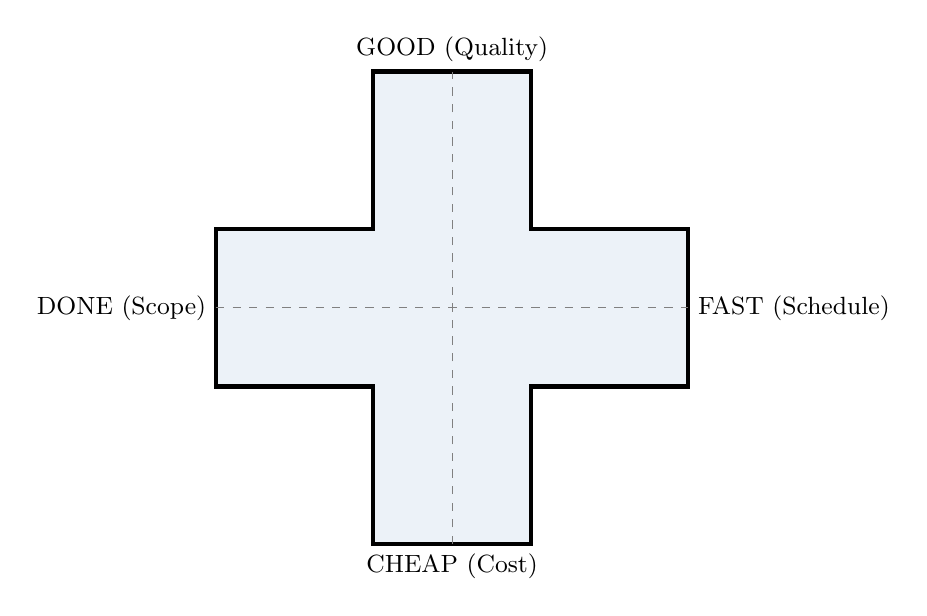
\begin{tikzpicture}[scale=2]
        % Definición de colores
        \definecolor{agileblue}{RGB}{70, 130, 180}
        
        % Dibujo de la cruz de 12 vértices (forma de "plus")
        \draw[line width=1.5pt, fill=agileblue!10] 
            (1,3) -- (2,3) -- (2,2) -- (3,2) -- (3,1) -- (2,1) -- 
            (2,0) -- (1,0) -- (1,1) -- (0,1) -- (0,2) -- (1,2) -- cycle;

        % Ejes internos (Las tensiones de la Cruz de Hierro)
        \draw[dashed, gray] (1.5,0) -- (1.5,3);
        \draw[dashed, gray] (0,1.5) -- (3,1.5);

        % Etiquetas de los extremos (Atributos de gestión)
        \node[above, font=\small] at (1.5,3) {GOOD (Quality)};
        \node[below, font=\small] at (1.5,0) {CHEAP (Cost)};
        \node[right, font=\small] at (3,1.5) {FAST (Schedule)};
        \node[left, font=\small] at (0,1.5) {DONE (Scope)};

    \end{tikzpicture}
    \caption{The Iron Cross of Software Development}
    \label{fig:iron-cross}
\end{figure}

There are two main questions whose answer (based on data, not on hope) is the main goal for Agile:
\begin{itemize}
    \item \emph{Do we do the right thing?}: Fast iterations, early feedback and planning are used.
    \item \emph{Can we still do it in time?}
\end{itemize}

Apart from that, some core Agile values are:
\begin{itemize}
    \item Personal courage and risk taking.
    \item Intense communication and collaboration, ignoring barriers of hierarchy, location and time.
    \item Rapid feedback and learning.
    \item Simplicity of code, design and teams.
    \item Respect.
\end{itemize}

There are different Agile methodologies, such as Scrum, Extreme Programming (XP), Crystal... However, they all share the same core values and principles, and they all aim to provide data to manage the iron cross of software development.

\section{Agile Methodologies}

\subsection{Scrum}

Scrum is one of the most popular Agile methodologies, and it is based on the idea of iterative and incremental development. A depper understanding of the concepts behind Scrum can be found in the Chapter 1 of the contents of the \myhref{https://losdeldgiim.github.io/subjects/Erasmus-DUE/Application\%20Management/Notes.pdf}{Application Management} course.

\subsection{XP (Extreme Programming)}

XP is another popular Agile methodology, and it is based on the idea of continuous feedback and improvement. In the Figure~\ref{fig:xp} we can see that it uses a planning and feedback loop that represents how frequent are the feedbacks and iterations in XP.
\begin{figure}
    \centering
    \includegraphics[width=0.5\textwidth]{./img/XP_Loop.png}
    \caption{Planning and feedback loops in XP}
    \label{fig:xp}
\end{figure}

This methodology is based on a concept named ``Circle of Life'', which represents the practices that should be taken, from a bigger aspect (the whole project) to a smaller aspect (the code itself). They will be convered in the following sections.

\subsubsection{Business-facing practices}

They are practices whose aim is to reduce the common gap between the business and the development team. The main goal here is planning correctly, and therefore a project should be divided into small pieces, where each piece should be estimated indivially. This estimation should be as accurate as possible but only as precise as needed. Some techniques for estimation are:
\begin{itemize}
    \item \ul{Trivariate Analysis}: Long-term estimation technique.
    % // TODO: Memorizar Trivariate Analysis
    The time to do a task is estimated based on three different scenarios:
    \begin{itemize}
        \item \emph{Worst case}: Time within which the task will be completed with a $95\%$ confidence.
        \item \emph{Nominal case}: Time within which the task will be completed with a $50\%$ confidence.
        \item \emph{Best case}: Time within which the task will be completed with a $5\%$ confidence.
    \end{itemize}


    \item \ul{Story Points}: Short-term estimation technique.
    % // TODO: Memorizar Story Points
    The project is divided in stories.
    \begin{itemize}
        \item An user story is an abbreviated description of a feature from the perspective of the user. It typically follows the format: ``As a [type of user], in order to [achieve a goal], I will [perform an action]''.
    \end{itemize}

    The stories should be made between the developpers and the stakeholders, and the details should be included when started working on the story, not before.\\

    Each story should be estimated in story points.
    \begin{itemize}
        \item A story point is a unit of measure for expressing the overall effort (not time) required to implement a user story.
    \end{itemize}
    
    An initial story (called the ``golden story'') of average complexity is chosen as a reference, and the other stories are estimated relative to it. For example, if the golden story is estimated to be 5 story points, and another story is estimated to be twice as complex, it would be assigned 10 story points. This technique allows for more accurate estimation and better planning of the project.\\

    Then, the project evolves in iterations (each one finishing with a demo), which are organized in interation planning meetings.
    \begin{itemize}
        \item In iteration planning meetings, the stakeholders select a set of user stories to be implemented in the next iteration, based on their priority and the team's \emph{velocity} (the number of story points the team can complete in an iteration).
    \end{itemize}

    The initial velocity is an initial guess, and the velocity of next iterations is calculated based on the velocity of the previous iteration. Managers may have a velocity chart, which is a visual representation of the team's velocity over time, to help track progress and make informed decisions about future iterations.

    In addition, a \emph{midpoint check} is usually done at the middle of the project, where the team reviews the story points completed so far, and compares it with the initial estimation. This allows to adjust the remaining story points asking the stakeholders to add/remove stories.
\end{itemize}

\subsubsection{Team-facing practices}

They are practices whose aim is to improve the communication and collaboration within the team. Some of these practices are:
\begin{itemize}
    \item Metaphore / Ubiquitous language: A common language that is used by all members of the team, including developers, testers, and stakeholders.
    \item Sustainable pace
    \item Collective ownership
    \item CI
    \item Standup meetings
\end{itemize}

\subsubsection{Technical practices}

They are practices whose aim is to improve the quality of the code and the design of the software. Some of these practices are:
\begin{itemize}
    \item TDD
    \item Pair programming: Two developers work together on the same code, sharing the workstation (it can also be done virtually). One developer writes the code, while the other reviews it in real-time. This practice promotes collaboration, knowledge sharing, helps to catch errors early in the development process, and also helps to train new team members. Pairing of larger teams can also be done, which is called \emph{mob programming}.
    
    Some characteristics that pair programming should have are:
    \begin{itemize}
        \item Optional
        \item Intermittent
        \item Unscheduled
        \item Short-lived
    \end{itemize}
    \item Refactoring
    \item Simple design
    
    Only the simplest design that works should be implemented. Some rules for simple design, in this priority order, are:
    \begin{enumerate}
        \item Pass all tests.
        \item Reveal the intention of the code.
        \item Remove duplication.
        \item Decrease the number of elements (classes, methods, variables...).
    \end{enumerate}
\end{itemize}